\documentclass[14pt,aspectratio=169]{beamer}

\usepackage{pgfpages}
\usepackage{fancyvrb}
\usepackage{pgfplots}

\usepackage{minted}
\usemintedstyle{tango}

\usepackage{amsfonts}

\usepackage{moresize}
\usepackage{anyfontsize}

\usepackage{tikz}
\usetikzlibrary{arrows,shapes}
\usetikzlibrary{arrows.meta}

\tikzstyle{process}=[rectangle, draw, thick, text width=5em, text centered, minimum height=2.5em, fill=gray!40]
\tikzstyle{entity}=[rounded rectangle, draw, thick, text width=5em, text centered, minimum height=1.5em, fill=gray!40]

\usetheme{auriga}
\usecolortheme{auriga}

\setbeamercolor{background canvas}{bg=lightgray}

% define some colors for a consistent theme across slides
\definecolor{red}{RGB}{181, 23, 0}
\definecolor{blue}{RGB}{0, 118, 186}
\definecolor{gray}{RGB}{146, 146, 146}

\title{Discrete Structures: \\ Ordered Pairs, Tuples, and Monoids in Python}

\author{{\bf Gregory M. Kapfhammer}}

\institute[shortinst]{{\bf Department of Computer Science, Allegheny College}}

\begin{document}

{
  \setbeamercolor{page number in head/foot}{fg=background canvas.bg}
  \begin{frame}
    \titlepage
  \end{frame}
}

%% Slide
%
\begin{frame}{Technical Question}
  %
  \hspace*{.25in}
  \begin{minipage}{5in}
  \begin{center}
    %
    {\large How do I employ the mathematical concepts of order pairs, n-tuples,
      monoids, and sequences to implement efficient Python programs that use
    higher-order functions with a clearly specified behavior?}
    %
  \end{center}
  \end{minipage}
  %
  \vspace{2ex}
  %
  \begin{center}
    %
    \small Let's learn how to translate concepts from discrete mathematics to
    implement efficient Python programs that are rigorously specified!
    %
  \end{center}
  %
\end{frame}

% Slide
%
\begin{frame}{Understanding Ordered Pairs}
  %
  \begin{itemize}
    %
    \item Mathematical concepts yield predictable programs
      %
      \vspace*{-.15in}
      %
    \item Understanding the concept of an ``ordered pair''
      %
      \begin{itemize}
        %
        \item {\bf Pair}: grouping of two entities
          %
        \item {\bf Ordered}: order of entities matters
          %
        \item {\bf Ordered Pair}: grouping of two entities for which order
          matters
          %
        \item {\bf Coordinate on Earth}: latitude and longitude are an ordered
          pair
          %
        \item {\bf Complex Numbers}: real and imaginary parts are an ordered
          pair
          %
        \item An ordered pair is not the same as a set of two elements!
          %
      \end{itemize}
      %
      \vspace*{-.2in}
      %
    \item If we have ordered pairs of entities, can we generalize to
      an ordered grouping beyond two entities? How?
      %
  \end{itemize}
  %
\end{frame}

% Slide
%
\begin{frame}[fragile]
  \frametitle{Practical Applications of Ordered Pairs}
  % \hspace*{-.15in}
  \begin{minipage}{6in}
    \vspace*{.25in}
    \begin{minted}[mathescape, numbersep=5pt, fontsize=\large]{text}
(40.758896° N, -73.985130° E)
  Times Square
(60.1699° N, 24.9384° E)
  Helsinki, Finland
(90.0° N, 0.0° E)
  North Pole
    \end{minted}
  \end{minipage}
  \vspace*{.05in}
  \begin{center}
    %
    \normalsize \noindent Latitude and longitude provide a ``global address''
    for a location\\
    %
    \normalsize \noindent Why does the order matter for these pairs of location
    data?\\
    %
  \end{center}
  %
\end{frame}

% Slide
%
\begin{frame}{Generalizing Ordered Pairs to n-Tuples}
  %
  \begin{itemize}
    %
    \item We could have an ``ordered triple'' or ``ordered quadruple''
      %
      \vspace*{-.15in}
      %
    \item The n-tuple is the collective name for ``tuples'' of any size
      %
      \begin{itemize}
        %
        \item A 2-tuple is the same as an ordered pair
          %
        \item A 3-tuple is the same as an ordered triple
          %
        \item A 4-tuple is the same as an ordered quadruple
          %
      \end{itemize}
      %
      \vspace*{-.2in}
      %
    \item Write n-tuples with notation like $(1,2)$ or $(x,y,z)$
      %
      \vspace*{-.2in}
    \item n-tuples enable creation of new mathematical objects
      %
      \vspace*{-.2in}
    \item n-tuples contain a finite number of entities
      %
      \vspace*{-.2in}
    \item While the type of entity in an n-tuple may be different, not
      every entity in the n-tuple must be different
      %
  \end{itemize}
  %
\end{frame}

% Slide
%
\begin{frame}[fragile]
  \frametitle{Defining n-Tuples in Python Programs}
  \normalsize
  % \hspace*{-.15in}
  \begin{minipage}{6in}
    \vspace*{.25in}
    \begin{minted}[mathescape, numbersep=5pt, fontsize=\large]{python}
pair = 3, 4
quadruple = "Story number", 3,
              "is", true
    \end{minted}
  \end{minipage}
  \vspace*{.25in}
  \begin{center}
    %
    \normalsize \noindent The same data type is not a requirement for a tuple \\
    \normalsize \noindent What are the data types of the values in these tuples? \\
    \normalsize \noindent Is there a more consistent way to encode these tuples? \\
    %
  \end{center}
  %
\end{frame}

% Slide
%
\begin{frame}[fragile]
  \frametitle{Details of n-Tuples in Python Programs}
  \normalsize
  \begin{minipage}{6in}
    \vspace*{.25in}
    \begin{minted}[mathescape, numbersep=5pt, fontsize=\large]{python}
pair = (3, 4)
quadruple = ("Story number", 3,
              "is", true)
    \end{minted}
  \end{minipage}
  \vspace*{.25in}
  \begin{center}
    %
    \normalsize \noindent Industry practice is to enclose tuples in parentheses \\
    \normalsize \noindent How does this make the discrete structure easier to
    read? \\
    \normalsize \noindent How does this make the Python program easier to debug? \\
    %
  \end{center}
  %
\end{frame}

% Slide
%
\begin{frame}[fragile]
  \frametitle{Special Tuples in the Python Language}
  \normalsize
  \begin{minipage}{6in}
    \vspace*{.25in}
    \begin{minted}[mathescape, numbersep=5pt, fontsize=\large]{python}
empty_tuple = ()
single_story = ("Story",)
single_number = (3,)
number = (3)
    \end{minted}
  \end{minipage}
  \vspace*{.25in}
  \begin{center}
    %
    \normalsize \noindent Some tuples may not (yet) contain any data in them! \\
    \normalsize \noindent Singleton tuples must use the comma notation\\
    \normalsize \noindent What is the difference between a tuple and a number? \\
    %
  \end{center}
  %
\end{frame}

% Slide
%
\begin{frame}[fragile]
  \frametitle{Packing and Unpacking Tuples in Python}
  \normalsize
  \begin{minipage}{6in}
    \vspace*{.25in}
    \begin{minted}[mathescape, numbersep=5pt, fontsize=\large]{python}
pair = (3,4)
x, y = pair
(x, y) = pair
x, y = y, x
(x, y) = (y, x)
    \end{minted}
  \end{minipage}
  \vspace*{.1in}
  \begin{center}
    %
    \normalsize \noindent You can ``pack'' and ``unpack'' n-tuples in Python! \\
    \normalsize \noindent Using optional parentheses improves readability \\
    \normalsize \noindent What is the purpose of the last two statements? \\
    %
  \end{center}
  %
\end{frame}

% Slide
%
\begin{frame}[fragile]
  \frametitle{Files in Directories Store n-Tuples}
  \begin{minipage}{6in}
    \vspace*{.15in}
    \begin{minted}[mathescape, numbersep=5pt, fontsize=\small]{text}
tylernelson@gmail.com,Careers adviser
gregory02@medina-mayer.com,"Accountant, management"
jonesmiguel@hotmail.com,Health and safety inspector
rsanchez@yahoo.com,"Surveyor, planning and development"
hillfrank@ward-wood.com,"Scientist, physiological"
aaronhunter@gmail.com,"Surveyor, insurance"
kylebarnes@hotmail.com,Records manager
joe70@yahoo.com,Network engineer
torresjames@white.info,Electrical engineer
shawkins@watson.com,Science writer
    \end{minted}
  \end{minipage}
  \vspace*{.05in}
  \begin{center}
    %
    \normalsize \noindent Comma separate value (CSV) are frequently used in
    business! \\
    %
    \normalsize \noindent Input this file of n-tuples into Python? Lists versus
    tuples? \\
    %
  \end{center}
  %
\end{frame}

% Slide
%
\begin{frame}[fragile]
  \frametitle{Parsing CSV Files in Python}
  \normalsize
  \begin{minipage}{6in}
    \vspace*{.25in}
    \begin{minted}[mathescape, numbersep=5pt, fontsize=\small]{python}
contacts_list = []
for contact_line in csv.reader(
    contacts.splitlines(),
    quotechar='"',
    delimiter=",",
    quoting=csv.QUOTE_ALL,
    skipinitialspace=True,
):
    current_contact_job = contact_line[1]
    if job_description in current_contact_job.lower():
        contacts_list.append(contact_line)
    \end{minted}
  \end{minipage}
  \vspace*{.1in}
  \begin{center}
    %
    \normalsize \noindent Use an iteration construct to create a list of
    contacts! \\
    %
  \end{center}
  %
\end{frame}

% Slide
%
\begin{frame}{Tuples are Worth Billions of Dollars!}
  %
  \begin{itemize}
    %
    \item Relational databases store tuples of data in rows
      %
      \vspace*{-.15in}
      %
    \item Introduction to relational databases
      %
      \begin{itemize}
        %
        \item Databases contain tables of data
          %
        \item A table consists of rows and columns
          %
        \item Each row of a table is an n-tuple
          %
        \item Database tables are specified by schemas
          %
        \item Schemas define the data types for the columns
          %
      \end{itemize}
      %
      \vspace*{-.2in}
      %
    \item Since CSV files do not offer enough structure or enforcement,
      relational databases provide an alternative in a relational database
      management system (RDBMS).
      %
  \end{itemize}
  %
\end{frame}

% Slide
%
\begin{frame}{Oracle Database Management System}
  %
  \begin{figure}
    \centering
    \includegraphics[scale=.0825]{images/oracle.png}
    \caption{The figure's caption}
  \end{figure}
  %
\end{frame}

% Slide
%
\begin{frame}{SQLite Database Management System}
  %
  \begin{figure}
    \centering
    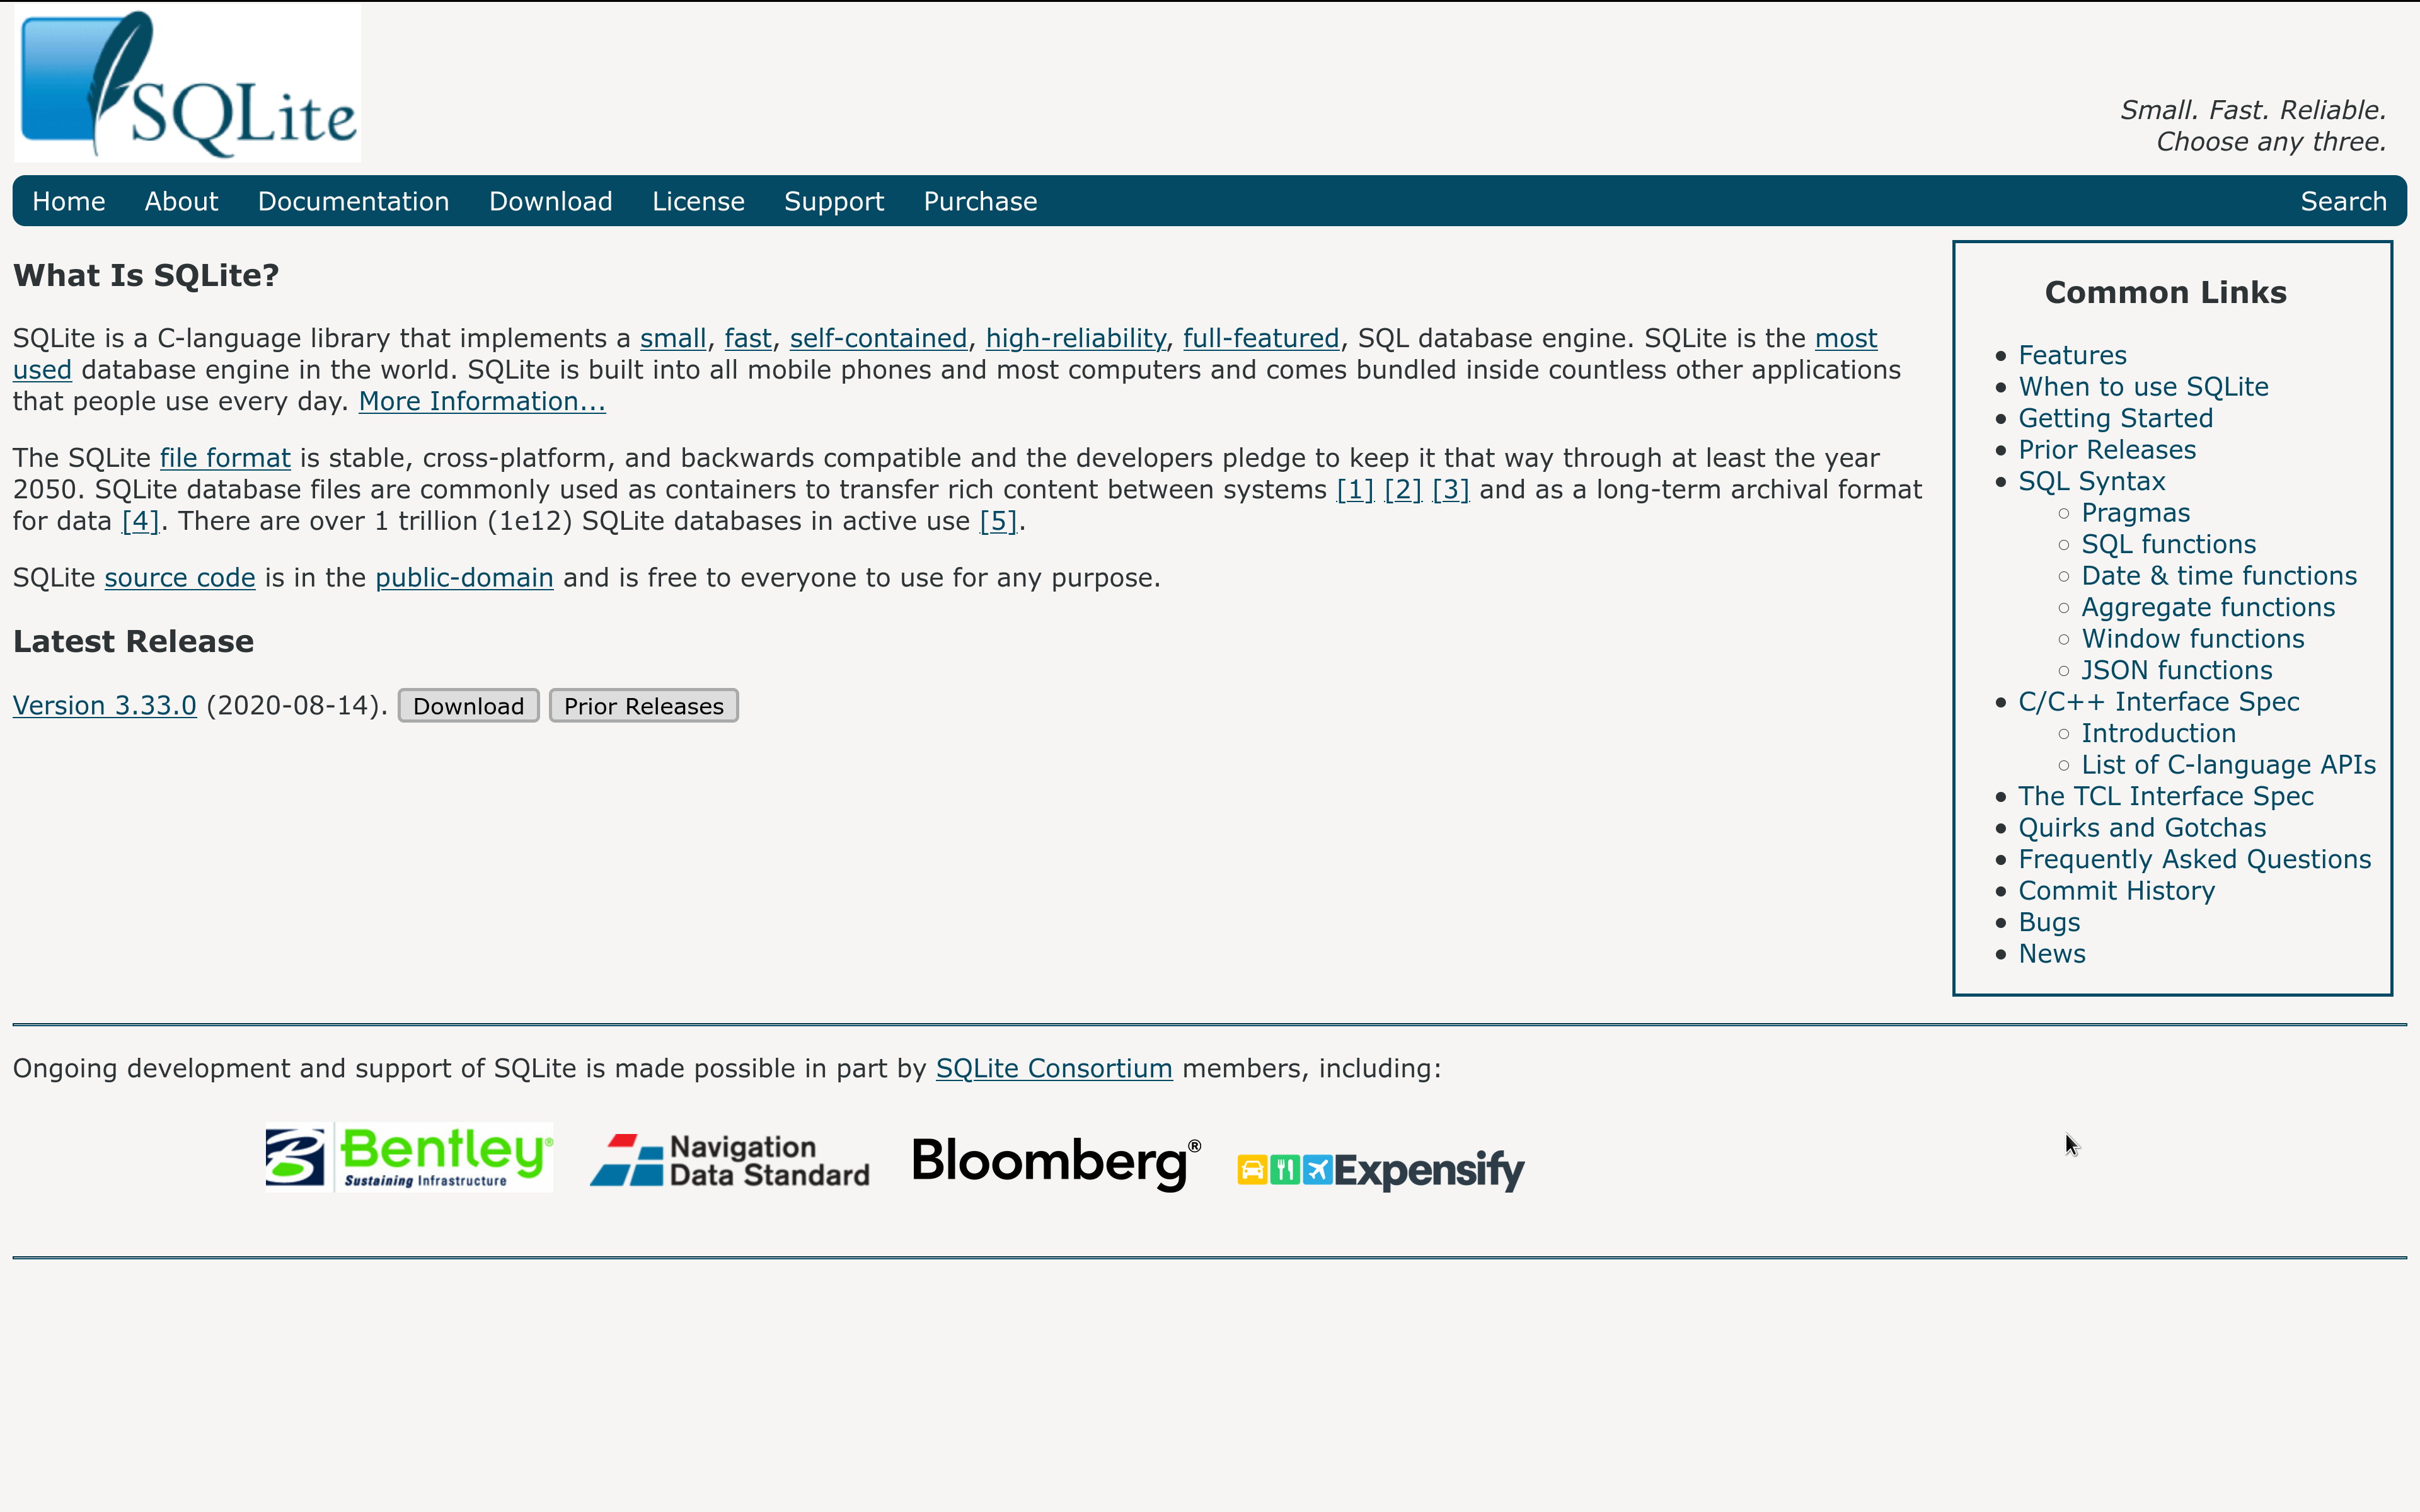
\includegraphics[scale=.0825]{images/sqlite.png}
    \caption{The figure's caption}
  \end{figure}
  %
\end{frame}

% Slide
%
\begin{frame}{Implementing and Debugging Python Functions}
  %
  \begin{itemize}
    %
    \item Use debugging statements to grasp a function's behavior!
      %
      \vspace*{-.15in}
      %
    \item Python functions to perform statistical analysis of data
      %
      \begin{itemize}
        %
        \item {\bf Q1}: How do you compute the median of a list of numbers?
          %
        \item {\bf Q2}: How do you compute the mode of a list of numbers?
          %
        \item {\bf Q3}: How do you compute a frequency table of a list of
          numbers?
          %
        \item {\bf Q4}: How do you compute the range of a list of numbers?
          %
        \item {\bf Q5}: How do you compute the variance and standard deviation?
          %
      \end{itemize}
      %
      \vspace*{-.2in}
      %
    \item Can you translate the mathematical descriptions of these summary
      statistics to Python programs? Can you ensure their correctness? Can you
      follow industry best practices?
      %
  \end{itemize}
  %
\end{frame}

\end{document}
